% \iffalse
\let\negmedspace\undefined
\let\negthickspace\undefined
\documentclass[journal,12pt,twocolumn]{IEEEtran}
\usepackage{cite}
\usepackage{amsmath,amssymb,amsfonts,amsthm}
\usepackage{algorithmic}
\usepackage{graphicx}
\usepackage{textcomp}
\usepackage{xcolor}
\usepackage{txfonts}
\usepackage{listings}
\usepackage{enumitem}
\usepackage{mathtools}
\usepackage{gensymb}
\usepackage{comment}
\usepackage[breaklinks=true]{hyperref}
\usepackage{tkz-euclide} 
\usepackage{listings}
\usepackage{gvv} 
\usepackage{caption}
\def\inputGnumericTable{}                   

%\usepackage[latin1]{inputenc}                                
\usepackage{color}                                            
\usepackage{array}                                            
\usepackage{longtable}                                       
\usepackage{calc}                                             
\usepackage{multirow}                                         
\usepackage{hhline}                                           
\usepackage{ifthen}                                           
\usepackage{lscape}

\newtheorem{theorem}{Theorem}[section]
\newtheorem{problem}{Problem}
\newtheorem{proposition}{Proposition}[section]
\newtheorem{lemma}{Lemma}[section]
\newtheorem{corollary}[theorem]{Corollary}
\newtheorem{example}{Example}[section]
\newtheorem{definition}[problem]{Definition}
\newcommand{\BEQA}{\begin{eqnarray}}
\newcommand{\EEQA}{\end{eqnarray}}
\newcommand{\define}{\stackrel{\triangle}{=}}
\theoremstyle{remark}
\newtheorem{rem}{Remark}

\begin{document}

\bibliographystyle{IEEEtran}
\vspace{3cm}

\title{NCERT 10.5.3 17Q}
\author{EE23BTECH11013 - Avyaaz$^{*}$% <-this % stops a space 
}
\maketitle
\newpage
\bigskip

\renewcommand{\thefigure}{\arabic{figure}}
\renewcommand{\thetable}{\arabic{table}}

\large\textbf{\textsl{Question:}}
In a school, students thought of planting trees in and around the school to reduce air
pollution. It was decided that the number of trees, that each section of each class will
plant, will be the same as the class, in which they are studying, e.g., a section of Class I
will plant $1$ tree, a section of Class II will plant $2$ trees and so on till Class $XII$. There are
three sections of each class. How many trees will be planted by the students?\\
\solution

From the above question, the number of trees planted by the students is in AP.
\begin{align}
 3, 6, 9, 12 .... 36   
\end{align}
\begin{table}[htbp]
\setlength{\extrarowheight}{8pt}
\centering
\begin{tabular}{|c|c|c|}
    \hline
    \textbf{Parameter} & \textbf{Description} & \textbf{Value} \\
    \hline
     \(x(0)\) & First Term &\(\dfrac{5}{2}\) \\
    \hline
     \(r\) = \(\dfrac{x(1)}{x(0)}\) & Common Ratio & \(\dfrac{1}{2}\) \\
    \hline
      \(x(n)\) & \(n^{th}\) Term & \(\dfrac{5}{2}\left(\dfrac{1}{2}\right)^n \cdot u(n)\) \\
    \hline
     \(x(19)\) & \(20^{th}\) Term &\(\dfrac{5}{2} \left(\dfrac{1}{2}\right)^{19}\) \\
    \hline
     \(u(n)\) &Unit step function & \\
    \hline
  \end{tabular}

\caption{Input Parameters}
\label{tab:parameter.10.5.3.17}
\end{table}

From \tabref{tab:parameter.10.5.3.17}:
\begin{align}
    x(n) = (3n+3)u(n)
\end{align}
Z-Transform of $x(n)$ : 
\begin{align}
    X(z) &= \frac{3z^{-1}}{\brak{1-z^{-1}}^2} + \frac{3}{\brak{1-z^{-1}}} ;|z| > 1\\
% \end{align}
% \begin{align}
 Y(z) &= X(z)U(z)\\
  &= \frac{3z^{-1}}{\brak{1-z^{-1}}^3} + \frac{3}{\brak{1-z^{-1}}^2}\\
    &= \frac{3z^{2}}{(z-1)^3} + \frac{3z^2}{(z - 1)^2};|z| > 1
    \end{align}
Using contour integration for inverse Z transformation,
\begin{align}
  y(11) &= \frac{1}{2\pi j}\int Y(z) z^{10} dz \\
         &= \frac{1}{2\pi j}\int \frac{3z^{12}}{(z-1)^{3}} dz + \frac{1}{2\pi j}\int \frac{3z^{12}}{(z-1)^{2}} dz\\
        \because R&=\frac{1}{\brak {m-1}!}\lim\limits_{z\to a}\frac{d^{m-1}}{dz^{m-1}}\brak {{(z-a)}^{m}f\brak z}\\
        R_1 &=\frac{1}{2!}\lim\limits_{z\to 1}\frac{d^2}{dz^2}\brak {(z-1)^3\frac{3z^{12}}{(z-1)^{3}}}\\
        &= 198\\
        R_2 &=\frac{1}{1!}\lim\limits_{z\to 1}\frac{d}{dz}\brak {(z-1)^2\frac{3z^{12}}{(z-1)^{2}}}\\
        &= 36\\
        \implies y(11) &= R_1 + R_2 \\
        &= 234   
\end{align}

\begin{figure}[htbp]
    \centering
    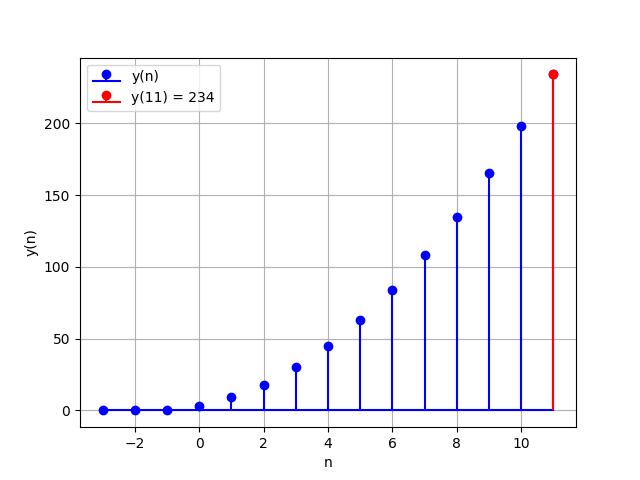
\includegraphics[width = \columnwidth]{figs/y(n)plot.png}
  \caption{}
    \label{fig:graph1}
\end{figure}

% \bibliographystyle{IEEEtran}
\end{document}
